\section{Auswertung}
\label{sec:Auswertung}
\subsection{Bestimmung der Apparatekonstante \texorpdfstring{$K_{gr}$}{math}}
\label{sec:BdA}
Zuerst wird mit der Gleichung \eqref{eqn:eta}
die Viskosität $\nu$ ermittelt.
Die Apparatekonstante ist für die kleine Kugel mit $K_{kl} = 7,64 \cdot 10^{-5}
\,\si{\milli\pascal\meter\tothe{3}\per\kilo\gram} $
gegeben. Im Folgenden wird die Dichte $\rho_{Fl}$ des destillierten Wassers, mit
1000 \si{\kilo\gram\per\meter\tothe{3}} angenommen. Mit der Gleichung
\begin{equation*}
  \rho_{K} = \frac{m}{\frac{4}{3}\pi\left(\frac{d}{2}\right)^3}
\end{equation*}
lässt sich die Dichte der beiden Kugeln bestimmen. Dabei bezeichnet $m$ das
Gewicht der Kugel und $d$ den Durchmesser der Kugel. Das Gewicht der Kugeln
beträgt 4,45 \si{\gram} für die kleine Kugel und 4,95 \si{\gram} für die große
Kugel. Für $d$ wird das Mittel aus den gemessenen Durchmesser genommen. Dann
ergibt sich für den Durchmesser der kleinen Kugel ca. $(0,01558 \pm 0.000002)$ \si{\meter} und
für die große Kugel ca. $(0,01575\pm 0.000001)$ \si{\meter}.
Die Messwerte  dazu sind in der Tabelle \ref{tab:dtab} dargestellt.
Daraus ergibt sich dann für die Dichte der kleinen Kugel $\rho_{kl} =
(2243.8 \pm 0.9) \si{\kilo\gram\per\meter\tothe{3}}$ und für die große Kugel
$\rho_{gr} = (2415.7 \pm 0.6) \si{\kilo\gram\per\meter\tothe{3}} $.
Schlussendlich ergibt sich dann
für die Viskosität, brechnet anhand der Daten der kleinen Kugel,
$(1.2084 \pm 0.0032)\si{\milli\pascal\second}$.
Aus der Gleichung \eqref{eqn:eta} folgt nun die Beziehung
\begin{equation*}
  K_{gr} = \frac{\eta}{(\rho_{gr} - \rho_{Fl})t_{gr}}
        = \frac{K_{kl} (\rho_{kl} - \rho_{Fl})t_{kl}}{(\rho_{gr} - \rho_{Fl})t_{gr}}\, ,
\end{equation*}
dabei bezeichnet $t_{kl}$ das Mittel der Fallzeit der kleinen Kugel und $t_{gr}$
das Mittel der Fallzeit der großen Kugel. Der Wert für $t_{kl}$ liegt bei
$(12.71 \pm 0.03) \si{\second}$ und für $t_{gr}$ bei $(85.84 \pm 0.22)
\si{\second}$.
Die Messwerte dazu sind in der Tabelle \ref{tab:t} dargestellt.
Daraus ergibt sich die Apparatekonstante $K_{gr}  = (9.94 \pm 0.04)
\cdot 10^{-6} \si{\milli\pascal\meter\tothe{3}\per\kilo\gram}$.
\begin{table}
  \centering
  \caption{Messwerte des ersten Versuchteils}
  \begin{subfigure}{0.48\textwidth}
    \centering
  \begin{tabular}{c c}
    \toprule
    $d_{kl} /\si{\milli\meter}$ & $d_{gr}/ \si{\milli\meter}$ \\
    \midrule
    15.59 & 15.76 \\
    15.58 & 15.76 \\
    15.59 & 15.755 \\
    15.59 & 15.76 \\
    15.59 & 15.76 \\
    \bottomrule
  \end{tabular}
  \caption{Gemessene Durchmesser für die kleine und große Kugel}
  \label{tab:dtab}
  \end{subfigure}
  \begin{subfigure}{0.48\textwidth}
    \centering
        \begin{tabular}{c c}
          \toprule
          $t_{kl} / \si{\second}$ & $t_{gr} / \si{\second} $\\
          \midrule
          12.69 & 87.07 \\
          12.55 & 86.09 \\
          12.75 & 86.09 \\
          12.81  & 86.38 \\
          12.8 & 85.9 \\
          12.73 & 85.63 \\
          12.82 & 84.81 \\
          12.75 & 85.46 \\
          12.74 & 86.18 \\
          12.52 & 84.83 \\
          \bottomrule
        \end{tabular}
        \caption{Gemessene Fallzeiten der kleinen und großen Kugel}
        \label{tab:t}
\end{subfigure}
\end{table}
\FloatBarrier
\subsection{Temperaturabhängigkeit der Viskosität}
Zuerst wird mit der Gleichung \eqref{eqn:eta} die Viskosität brechnet, logarithmiert
und gegen $\frac{1}{T}$ aufgetragen, hierbei ist $T$ natürlich die Temperatur.
Wird nun eine Ausgleichrechnung mit
\begin{equation*}
  \symup{ln}(\eta)= \frac{B}{T}\cdot\symup{ln}(A)
\end{equation*}
durchgeführt, so ergibt sich die Konstante $ A =  (0.00377 \pm 0.00032)
\si{\milli\pascal\second}$ und $B = (1681 \pm 23) \si{\kelvin}$, hier wurde
die Ausgleichsrechnung mit Python und Scipy \cite{scipy} durchgeführt. Der soeben
beschriebene Vorgang ist in Abbildung \ref{fig:plot} dargestellt.
\begin{figure}
  \centering
  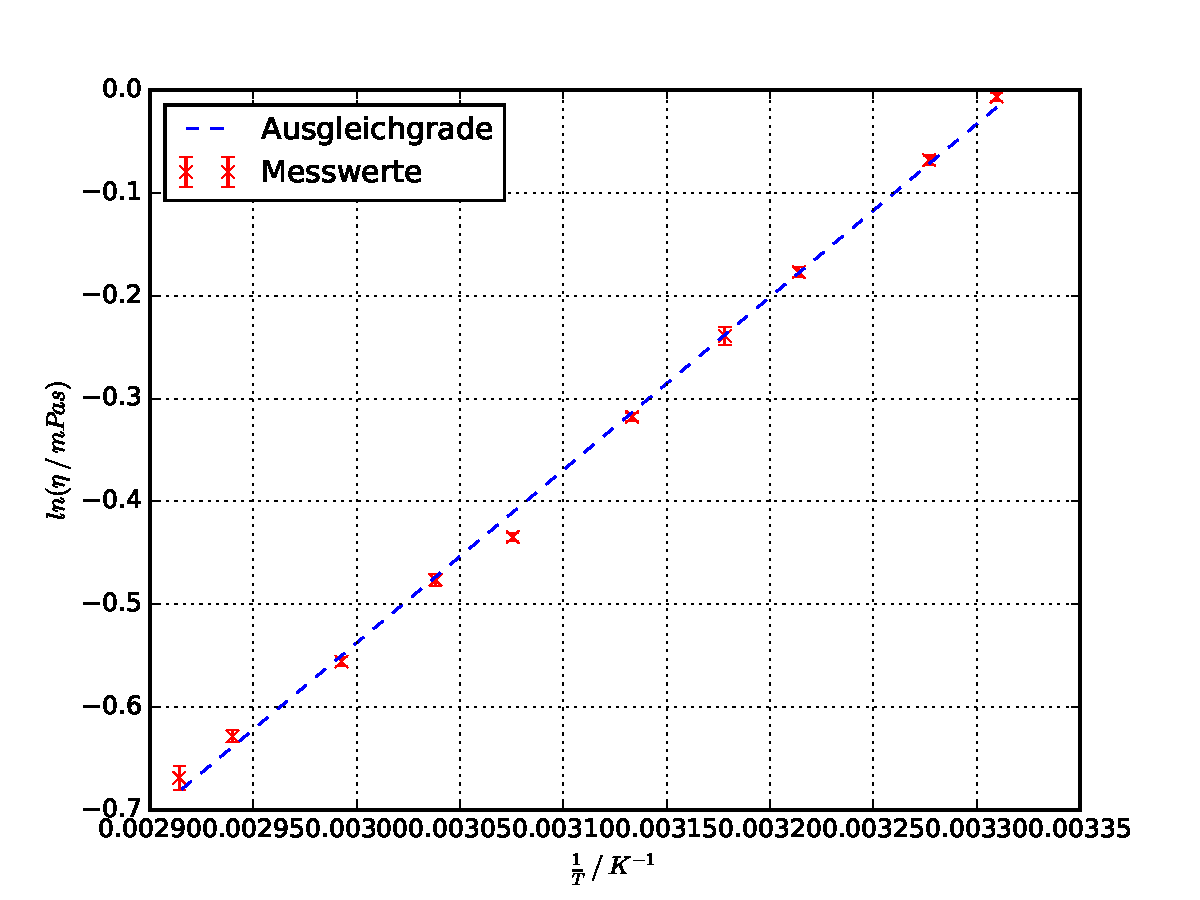
\includegraphics[height= 7cm]{Plots/plot.pdf}
  \caption{Temperaturabhängigkeit der Viskosität}
  \label{fig:plot}
\end{figure}
Die oben genannte Gleichung zur Ausgleichsrechnung kommt von der Andradeschen
Gleichung \eqref{eqn:eta(T)}, diese beschreibt die Temperaturabhängigkeit der
Viskosität.
Dabei ist zu beachten,
dass das destillierte Wasser seine Dichte mit der Temperatur ändert. Deshalb
werden nur Werte in die Ausgleichsrechnung, sowie in der Brechnung der
Viskosität einbezogen, die den Signifikanzbereich nicht verletzen.
\begin{table}
  \centering
  \caption{Werte des Diagramms}
  \sisetup{round-mode = places , round-precision = 2}
  \begin{tabular}{S S S}
    \toprule
    $ \frac{1}{T} / \si{\kelvin} $ &
    ln $\text{(}\eta / \si{\milli\pascal\meter}\text{)}$  &
     ln $\text{(}\Delta \eta / \si{\milli\pascal\meter}\text{)}$  \\
    \midrule
         3.309614429918914490e-03 & -6.570905882970178025e-03 & 4.034219172099570185e-03\\
         3.277076847452072787e-03 & -6.822776413331044232e-02 & 4.535995114083736512e-03\\
         3.213883978788366173e-03 & -1.770184984026798858e-01 & 4.825170317944159001e-03\\
         3.178134435086604325e-03 & -2.391459711890263906e-01 & 8.528064368417862320e-03\\
         3.133322888923703760e-03 & -3.177890985081395780e-01 & 3.735834430886281025e-03\\
         3.075503613716746524e-03 & -4.346054835334280386e-01 & 4.283181366968836015e-03\\
         3.038128512836093219e-03 & -4.762203647690622099e-01 & 5.757571901077946155e-03\\
         2.992667963489451053e-03 & -5.557910403356511875e-01 & 4.180174685403765904e-03\\
         2.939879464941937658e-03 & -6.284277027585306596e-01 & 5.911504513955105622e-03\\
         2.914177473408130839e-03 & -6.688154774523018542e-01 & 1.146343641715576525e-02\\

     \bottomrule
  \end{tabular}
  \label{tab:plot}
\end{table}

\subsection{Reynolds-Zahl}
Die Reynolds-Zahl \cite{wiki} ist definiert durch
\begin{equation*}
  Re = \frac{\rho\cdot s\cdot d}{\eta \cdot t}.
\end{equation*}
Dabei bezeichnet $\rho$ die Dichte des Mediums $v$ die Strömungsgeschwindigkeit,
$d$ der Durchmesser des Rohrs und $\eta$ die Viskosität.
Da das destillierte Wasser nicht
strömt, wird hier die Fallgeschwindigkeit der Kugel benutzt.
Für die Werte aus Kapitel \ref{sec:BdA} ergibt sich
für die kleine Kugel $Re = (50.72 \pm 0.26)$ und für die große Kugel
$ Re = (7.596 \pm 0.026) $.Die Reynolds-Zahl für die große Kugel bei 70 \si{\celsius}
beträgt $(113.4 \pm 1.4)$. Da diese Zahlen wesentlich kleiner sind als
1150 kann von einer laminaren Strömung ausgegangen werden.
\begin{table}
  \centering
  \caption{Messwerte zur Temperaturabhängigkeit der Viskösität}
  \sisetup{round-mode = places , round-precision = 2}
  \scalebox{0.9}{
  \begin{tabular}{S[fixed-exponent= 0,
  scientific-notation = fixed] S[fixed-exponent= 0,
  scientific-notation = fixed] S[fixed-exponent= 0,
  scientific-notation = fixed] S[fixed-exponent= 0,
  scientific-notation = fixed] S S[fixed-exponent= 0,
  scientific-notation = fixed] S}
    \toprule
    $T / \si{\kelvin}$ & $t_{1} / \si{\second}$ & $t_{2} / \si{\second}$ &
    $ t_{Mittel} / \si{\second} $ & $\Delta t_{Mittel} / \si{\second}$
    &$ \eta /\si{\milli\pascal\meter}$ & $ \Delta \eta /\si{\milli\pascal\meter}$ \\
    \midrule
    3.021499999999999773e+02 & 7.068999999999999773e+01 & 7.045999999999999375e+01 & 7.057499999999998863e+01 & 1.150000000000019756e-01 & 9.934506353115464261e-01 & 4.007797599508338381e-03\\
    3.051499999999999773e+02 & 6.618000000000000682e+01 & 6.653000000000000114e+01 & 6.635500000000000398e+01 & 1.749999999999971578e-01 & 9.340477067814052514e-01 & 4.236835834281573940e-03\\
    3.111499999999999773e+02 & 5.970000000000000284e+01 & 5.932999999999999829e+01 & 5.951500000000000057e+01 & 1.850000000000022460e-01 & 8.377642870785221296e-01 & 4.042355371444933919e-03\\
    3.146499999999999773e+02 & 5.550000000000000000e+01 & 5.635999999999999943e+01 & 5.592999999999999972e+01 & 4.299999999999997158e-01 & 7.872999508745986974e-01 & 6.714144658310799117e-03\\
    3.191499999999999773e+02 & 5.172999999999999687e+01 & 5.167000000000000171e+01 & 5.170000000000000284e+01 & 2.999999999999758069e-02 & 7.277562571109735812e-01 & 2.718776882608103795e-03\\
    3.251499999999999773e+02 & 4.610000000000000142e+01 & 4.589999999999999858e+01 & 4.600000000000000000e+01 & 1.000000000000014211e-01 & 6.475200740252375908e-01 & 2.773445915803179201e-03\\
    3.291499999999999773e+02 & 4.392999999999999972e+01 & 4.432000000000000028e+01 & 4.412500000000000000e+01 & 1.950000000000002842e-01 & 6.211265927470349668e-01 & 3.576181017412614210e-03\\
    3.341499999999999773e+02 & 4.067000000000000171e+01 & 4.082999999999999829e+01 & 4.075000000000000000e+01 & 7.999999999999829470e-02 & 5.736183264462703102e-01 & 2.397824807294372199e-03\\
    3.401499999999999773e+02 & 3.771999999999999886e+01 & 3.807000000000000028e+01 & 3.789499999999999602e+01 & 1.750000000000007105e-01 & 5.334298522866603998e-01 & 3.153372979670998177e-03\\
    3.431499999999999773e+02 & 3.678999999999999915e+01 & 3.600000000000000000e+01 & 3.639499999999999602e+01 & 3.949999999999995737e-01 & 5.123150672640982561e-01 & 5.872891199132868924e-03\\
    \bottomrule
  \end{tabular}
  }
\end{table}



























%
